\iffalse
\chapter{2016}
\author{AI24BTECH11015 - Harshvardhan Patidar}
\section{ph}
\fi
\item[] \textbf{Q.\ref{1} - Q.\ref{5} carry one mark each.}
% \begin{enumerate}
    \item \label{1} The volume of a sphere of diameter $1$ unit is \_\_\_\_\_\_\_\_ than the volume of a cube of side $1$ unit.
        \begin{enumerate}
            \item least
            \item less
            \item lesser
            \item low
        \end{enumerate}

    \item The unruly crowd demanded that the accused be \_\_\_\_\_\_\_\_ without trial.
        \begin{enumerate}
            \item hanged
            \item hanging
            \item hankering
            \item hung
        \end{enumerate}

    \item Choose the statement(s) where the underlined word is used correctly:
        \begin{itemize}
            \item[(i)] A \underline{prone} is a dried plum.
            \item[(ii)] He was lying \underline{prone} on the floor.
            \item[(iii)] People who eat a lot of fat are \underline{prone} to heart disease.
        \end{itemize}
        \begin{enumerate}
            \item (i) and (iii) only
            \item (iii) only
            \item (i) and (ii) only
            \item (ii) and (iii) only
        \end{enumerate}

    \item \textbf{Fact:} If it rains, then the field is wet. \\ \\ Read the following statements:
        \begin{itemize}
            \item[(i)] It rains
            \item[(ii)] The field is not wet
            \item[(iii)] The field is wet
            \item[(iv)] It did not rain
        \end{itemize}

        Which one of the options given below is \textbf{NOT} logically possible, based on the given fact?
        \begin{enumerate}
            \item If (iii), then (iv).
            \item If (i), then (iii).
            \item If (i), then (ii).
            \item If (ii), then (iv).
        \end{enumerate}    
    \item \label{5} A window is made up of a square portion and an equilateral triangle portion above it. The base of the triangular portion coincides with the upper side of the square. If the perimeter of the window is $6 m$, the area of the window in $m^2$ is \_\_\_\_\_\_\_\_.
        \begin{enumerate}
            \item $1.43$
            \item $2.06$
            \item $2.68$
            \item $2.88$
        \end{enumerate}

        \item[] \textbf{Q.\ref{6} - Q.\ref{10} carry two marks each.}
    \item \label{6} Students taking an exam are divided into two groups, \textbf{P} and \textbf{Q} such that each group has the same number of students. The performance of each of the students in a test was evaluated out of $200$ marks. It was observed that the mean of group \textbf{P} was $105$, while that of group \textbf{Q} was $85$. The standard deviation of group \textbf{P} was $25$, while that of group \textbf{Q} was $5$. Assuming that the marks were distributed on a normal distribution, which of the following statements will have the highest probability of being \textbf{TRUE}?
        \begin{enumerate}
            \item No student in group \textbf{Q} scored less marks than any student in group \textbf{P}
            \item No student in group \textbf{P} scored less marks than any student in group \textbf{Q}
            \item Most students of group \textbf{Q} scored marks in a narrower range than students in group \textbf{P}.
            \item The median of the marks of group \textbf{P} is $100$.
        \end{enumerate}

    \item A smart city integrates all modes of transport, uses clean energy and promotes sustainable use of resources. It also uses technology to ensure safety and security of the city, something which critics argue, will lead to a surveillance state. \\ \\ Which of the following can be logically inferred from the above paragraph?
        \begin{itemize}
            \item [(i)] All smart cities encourage the formation of surveillance states.
            \item [(ii)] Surveillance is an integral part of a smart city.
            \item [(iii)] Sustainability and surveillance go hand in hand in a smart city.
            \item [(iv)] There is a perception that smart cities promote surveillance.
        \end{itemize}

        \begin{enumerate}
            \item (i) and (iv) only
            \item (ii) and (iii) only
            \item (iv) only
            \item (i) only
        \end{enumerate}

    \item Find the missing sequence in the letter series. \\ \\ B, FH, LNP, \_\_\_\_.
        \begin{enumerate}
            \item SUWY
            \item TUVW
            \item TVXZ
            \item TWXZ
        \end{enumerate}

    \item The binary operation $\Box$ is defined as $a \Box b = ab+\brak{a+b}$, where $a$ and $b$ are any two real numbers. The value of the identity element of this operation, defined as the number $x$ such that $a \Box x = a$, for any $a$, is \_\_\_\_\_\_\_\_.
        \begin{enumerate}
            \item $0$
            \item $1$
            \item $2$
            \item $10$
        \end{enumerate}

    \item \label{10} Which of the following curves represents the function $y = \ln\brak{\abs{e^{\sbrak{\abs{\sin \brak{\abs{x}}}}}}}$ for $\abs{x} < 2\pi$? Here, $x$ represents the abscissa and $y$ represents the ordinate.
        \begin{multicols}{2}
        \begin{enumerate}
            \item 
            \begin{figure}[H]
                \centering
                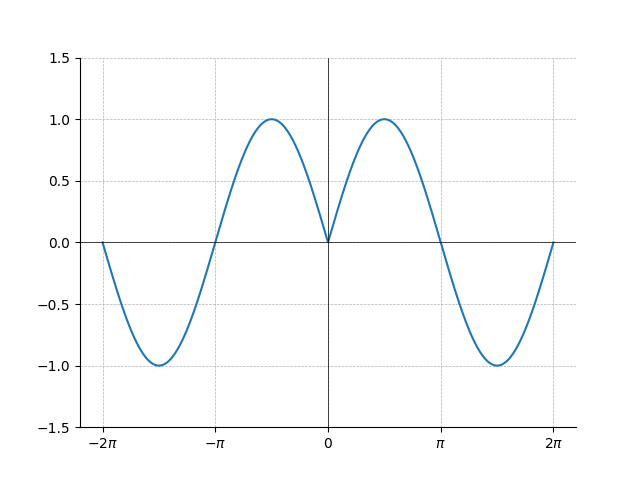
\includegraphics[width = 1\linewidth]{Gate-yearwise/AI24BTECH11015/figs/10a.png}
                \caption{}
            \end{figure}
            \item 
            \begin{figure}[H]
                \centering
                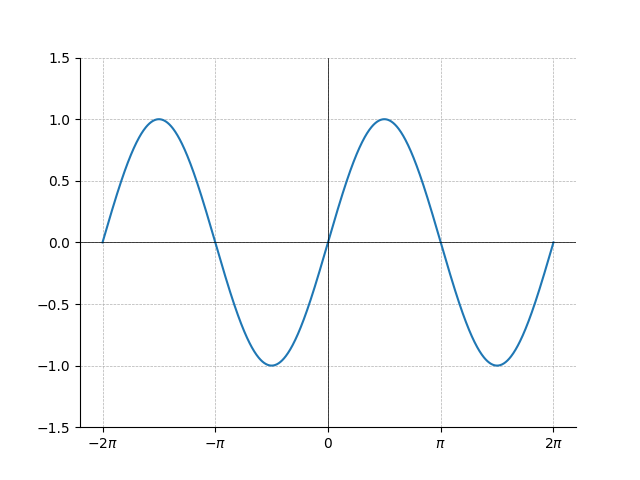
\includegraphics[width = 1\linewidth]{Gate-yearwise/AI24BTECH11015/figs/10b.png}
                \caption{}
            \end{figure}
            \item 
            \begin{figure}[H]
                \centering
                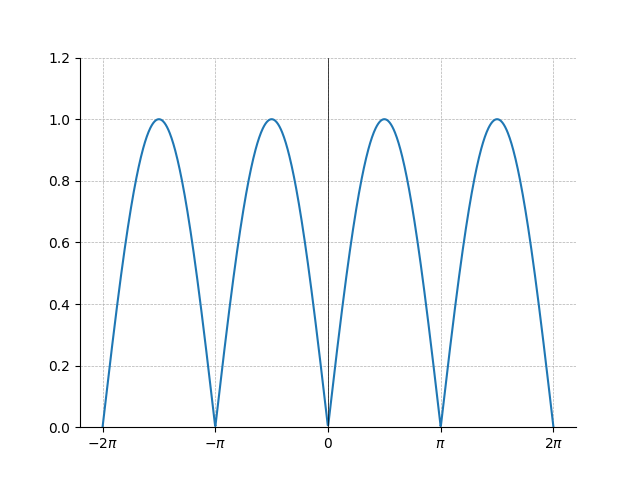
\includegraphics[width = 1\linewidth]{Gate-yearwise/AI24BTECH11015/figs/10c.png}
                \caption{}
            \end{figure}
            \item 
            \begin{figure}[H]
                \centering
                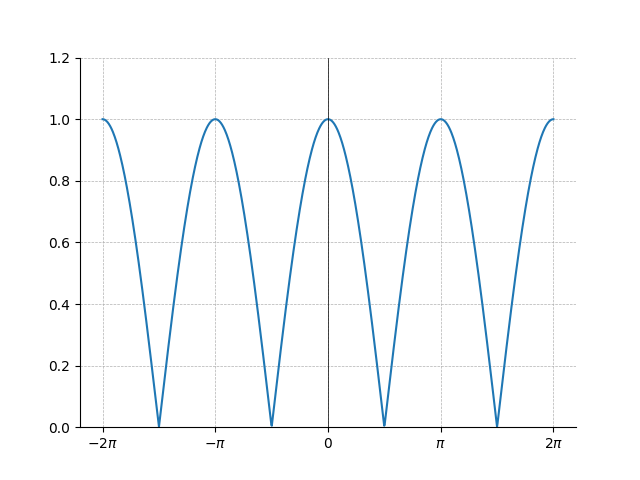
\includegraphics[width = 1\linewidth]{Gate-yearwise/AI24BTECH11015/figs/10d.png}
                \caption{}
            \end{figure}
        \end{enumerate}
    \end{multicols}

        \item[] \textbf{Q.\ref{11} - Q.10.25 carry one mark each}
    \item \label{11} Consider the linear differential equation $\frac{dy}{dx} = xy$. If $y=2$ at $x=0$, then the value of $y$ at $x=2$ is given by
        \begin{enumerate}
            \item $e^{-2}$
            \item $2e^{-2}$
            \item $e^{2}$
            \item $2e^{2}$
        \end{enumerate}

    \item Which of the following magnetic vector potentials gives rise to a uniform magnetic field $B_0 \hat{k}$?
        \begin{enumerate}
            \item $B_0 z \hat{k}$
            \item $- B_0 x \hat{j}$
            \item $\frac{B_0}{2} \brak{-y \hat{i} + x \hat{j}}$
            \item $\frac{B_0}{2} \brak{y \hat{i} + x \hat{j}}$
        \end{enumerate}

    \item The molecule $^{17}O_2$ is
        \begin{enumerate}
            \item Raman active but not NMR (nuclear magnetic resonance) active.
            \item Infrared active and Raman active but not NMR active.
            \item Raman active and NMR active.
            \item Only NMR active.
        \end{enumerate}
% \end{enumerate}

